\documentclass[12pt]{beamer}
\usetheme{metropolis}
\definecolor{myblue}{RGB}{34, 70, 135}
\setbeamercolor{frametitle}{fg=white}
\usepackage{listings}
\lstset{
  basicstyle=\ttfamily\small,
  keywordstyle=\color{myblue}\bfseries,
  commentstyle=\color{gray},
  stringstyle=\color{orange},
  showstringspaces=false,
  frame=lines,
  columns=fullflexible,
}
\usepackage{tikz}
\usetikzlibrary{shadows}
\begin{document}
% Stunning Title Slide
{
\begin{frame}[plain]
  \vfill
  \centering
  {\usebeamerfont{title}\usebeamercolor[fg]{title}\Huge \textbf{Cross-Religion Center Location}\par}
  \vskip1em
  {\usebeamerfont{subtitle}\large Location assignment of a Cross Religion Center Using ML \LaTeX\par}
  \vskip2em
  {\usebeamerfont{author}\large Nikos Nteits\par}

  \vskip2em
  {\usebeamerfont{date}\normalsize \today\par}
  \vfill


\end{frame}
}
\begin{frame}{Agenda}
\tableofcontents
\end{frame}

\section{Outlline of the Problem}

\begin{frame}{Outline}

The aim of this analysis is to provide the optimal location \\
of a Cross Religion Center in the United States of America. \\
The location should promote interfaith dialogue and minimize traveling costs for the faithfull. 
This will be achieved by placing it in a location that minimizes its geographical distance from every Church taking into account the number of faithfull that are registered in the respective Church.



\end{frame}



\section{The Dataset}

\begin{frame}{Dataset}

The dataset contains information about populations of churches per county of the United States of America. It consists of 3075 rows ( counties ) and 235 columns.



\begin{itemize}

  	\item  \textbf{CaseID} : an id for the entry
	\item \textbf{CNAME} : an id for the entry
	\item  \textbf{STCODE} : an id for the entry
	\item  \textbf{CCODE} : an id for the entry
	\item  \textbf{TOTPOP} : an id for the entry
	\item  \textbf{TOTMEMB} : an id for the entry

\end{itemize}
\end{frame}
\begin{frame}{Dataset}

The dataset contains information about populations of churches per county of the United States of America. It consists of 3075 rows ( counties ) and 235 columns.



\begin{itemize}


	\item  Columns that end with ‘M’ eg : AOG\_M, denoting the number of members of Church AOG in the County.
	\item  Columns that end with ‘C’ eg : AOG\_C, denoting the number of Churches AOG in the County.
\end{itemize}
TOTCHUR and Columns that end with  ‘\_C’ will be discarded as only the population will be used to determine the location of the cross religion center.




\end{frame}
\section{EDA}
\begin{frame}{EDA}




\begin{center}
    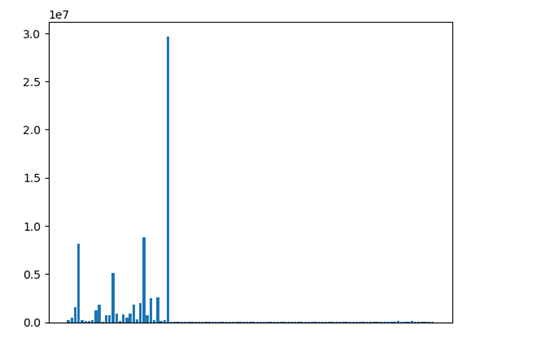
\includegraphics[width=0.7\linewidth]{barplot.png}
    
    % Example legend below the image
    \vspace{1em}
    \begin{tabular}{ll}
      \textcolor{black}{ Total population per Church }\\

      % Add more as needed
    \end{tabular}
\end{center}




\end{frame}



\begin{frame}{EDA}


Total Population per Church
\vspace{0.1cm}

 \textbf{CATH\_M}     29688058\\
 \textbf{METH\_M}     8790025\\
 \textbf{SBC\_M}      8121069\\
 \textbf{JEWS\_M}      5112024\\
 \textbf{EPISC\_M}    2544320\\

\vspace{0.4cm}
Catholic, Methodist, Southern Baptists, Jews and Protestant Episcopal 
Church are the 5 most populated churches. 






\end{frame}


\begin{frame}{EDA}



Cherokee.AL, Madison.IL and Fresno.CA have the highest per-person ratio of Orthodox Christian members.
\begin{center}
    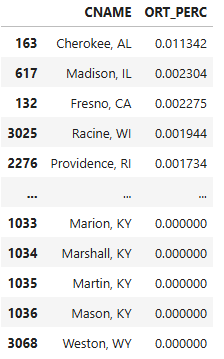
\includegraphics[width=0.8\linewidth, height=0.6\textheight, keepaspectratio]{Cname_ort.png}
    
    % Example legend below the image
    \vspace{1em}
    \begin{tabular}{ll}
      \textcolor{black}{ Per-person ratio of Orthodox 
 Christian members
 }\\

      % Add more as needed
    \end{tabular}
\end{center}




\end{frame}


\begin{frame}{EDA}
The 3 most extreme counties with respect to the distribution of their churches across religions (LOF).



 \textbf{Hinsdale, CO}     \\
 \textbf{Kings, NY}     \\
 \textbf{Billings, ND}      \\









\end{frame}






\section{Analysis}

\begin{frame}{Analysis  }

A Cross-Religion Center should be located in an area with high religious diversity to ensure representation and inclusivity. It must be geographically central for accessibility to a large portion of the population and minimize transportation.












\end{frame}


\begin{frame}{Analysis  }



\begin{itemize}
\item \textbf{Step 1 :} Build hypothetical per Religion centers with the use of weighted k-Means with 1 centroid where weights will be the population of every county for the specified religion .
\item \textbf{Step 2 :} Perform weighted  k-Means with 1 centroid to the per Religion centers , this time the weights will be the total Religion population .



\end{itemize}










\end{frame}

\section{Results}
\begin{frame}{Results}


Results for per religion centroids are :
\begin{center}
    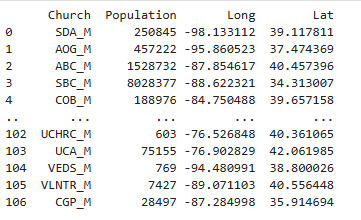
\includegraphics[width=0.8\linewidth, height=0.6\textheight, keepaspectratio]{Centroids.png}
    
    % Example legend below the image
    \vspace{1em}
    \begin{tabular}{ll}
      \textcolor{black}{Per Religion Churches
 }\\

      % Add more as needed
    \end{tabular}
\end{center}
\end{frame}

\begin{frame}{Results}


Results for the coordinates of the Cross-Religion Center are  :
\begin{center}
    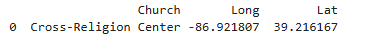
\includegraphics[width=0.8\linewidth, height=0.6\textheight, keepaspectratio]{Final_Centroid.png}
    
    % Example legend below the image
    \vspace{1em}
    \begin{tabular}{ll}
      \textcolor{black}{Per Religion Churches
 }\\

      % Add more as needed
    \end{tabular}
\end{center}
\end{frame}

\begin{frame}{Visual Representation}
 For the visualization purposes an interactive Dash app was built. In the first plot one can see a heatmap of the population of every church along with the centroid derived from the first weighted k-Means.
 Churches can be changed through the scrollbar. In the second plot one can see every centroid, with size depending on the total population of each church, along with a red star which is the proposed location of the cross religious center.



 
\end{frame}
\section{Visual Representation}
\begin{frame}{Visual Representation}


Heatmap with the location of the virtual centoid for ALUTH\_M
\begin{center}
    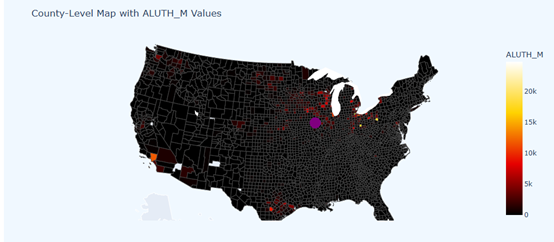
\includegraphics[width=0.8\linewidth, height=0.6\textheight, keepaspectratio]{C_level_map.png}
    
    % Example legend below the image
    \vspace{1em}
    \begin{tabular}{ll}
      \textcolor{black}{Per Religion Churches
 }\\

      % Add more as needed
    \end{tabular}
\end{center}

\end{frame}


\begin{frame}{Visual Representation}


Location of the Virtual Religion Centers and the Cross Religio Center 
\begin{center}
    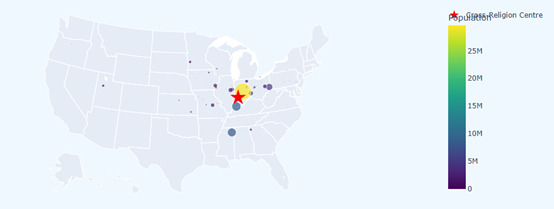
\includegraphics[width=0.8\linewidth, height=0.6\textheight, keepaspectratio]{Star.png}
    
    % Example legend below the image
    \vspace{1em}
    \begin{tabular}{ll}
      \textcolor{black}{Per Religion Churches
 }\\

      % Add more as needed
    \end{tabular}
\end{center}

\end{frame}






\end{document}

